Die Zeit $t$ wird ab dem Start des ersten Autos gezählt, $\tau = t-\Delta t$ ist die Zeit seit der Durchfahrt des zweiten Autos an der Startlinie. Die Orte der Autos sind
\begin{align}
 s_1 &= \frac{1}{2}a_1\,t^2 = \frac{1}{2}a_1\left(\tau+\Delta t\right)^2, \qquad s_2 = v_2\,\tau+\frac{1}{2}a_2\,\tau^2
\end{align}
Aus $s_1 = s_2$ folgt die quadratische Gleichung
\begin{align}
 \frac{1}{2}\left(a_2-a_1\right)\tau^2+\left(v_2-a_1\Delta t\right)\tau-\frac{1}{2}a_1\Delta t^2 &= 0
\end{align}
Die positive Lösung ist
\begin{align}
 \tau &= \tauRF
\end{align}
Mit $v_2-a_1\Delta t = \vRb-\aRa\cdot\dtR = \pR$ ergibt sich
\begin{align}
 \tau &= \frac{-\pR+\sqrt{\left(\pR\right)^2+\left(\aRb-\aRa\right)\cdot\aRa\cdot\left(\dtR\right)^2}}{\aRb-\aRa} = \tauR
\end{align}
Das zweite Auto holt das erste also
\begin{align}
 t &= \tRF = \tauR+\dtR = \tR \approx \result{\tRP{0}{2}}
\end{align}
nach dem Start des ersten Autos ein, und zwar im Abstand
\begin{align}
 s &= \sRF = \frac{1}{2}\cdot\aRa\cdot\left(\tR\right)^2 = \sR \approx \result{\sRP{0}{2}}
\end{align}
von der Startlinie.

\begin{center}
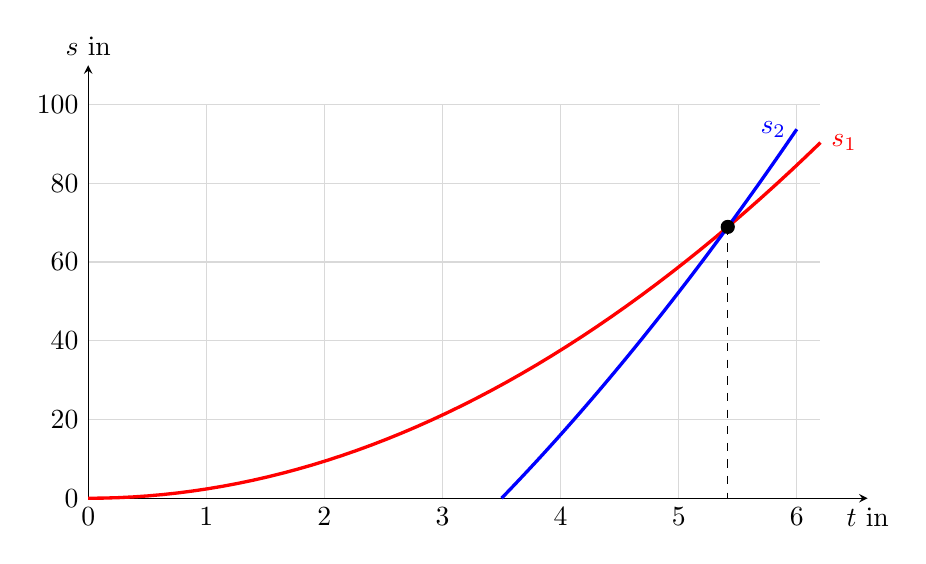
\begin{tikzpicture}[>=stealth, xscale=1.5, yscale=0.05]
 \foreach \x in {1,...,6} \draw[gray!30] (\x,0) -- (\x,100);
 \foreach \y in {20,40,...,100} \draw[gray!30] (0,\y) -- (6.2,\y);
 \draw[->] (0,0) -- (6.6,0) node[below] {$t$ in \si{\second}};
 \draw[->] (0,0) -- (0,110) node[above] {$s$ in \si{\meter}};
 \foreach \x in {0,...,6} \node[below] at (\x,0) {\x};
 \foreach \y in {0,20,...,100} \node[left] at (0,\y) {\y};
 \draw[red, very thick, domain=0:6.2, samples=50] plot (\x, {2.35*\x*\x}) node[right] {$s_1$};
 \draw[blue, very thick, domain=3.5:6.0, samples=50] plot (\x, {31*(\x-3.5)+2.6*(\x-3.5)*(\x-3.5)}) node[left] {$s_2$};
 \fill (5.415,68.92) ellipse (0.06 and 1.8);
 \draw[dashed] (5.415,68.92) -- (5.415,0);
\end{tikzpicture}
\end{center}
